% \chapter{Evaluation}
%
% This chapter evaluates the implemented pipeline against the two primary claims stated in the research objectives: the ability to sustain high-throughput ingestion across all monitored cities, and the delivery of end-to-end latency below one minute from sensor reading generation to stored aggregate.
%
% \section{Experimental Setup}
%
% All experiments were conducted on a single host machine (Apple M-series, X GB RAM) running all pipeline services via Docker Compose. No external infrastructure was used. The data source was a historical Parquet file replayed at configurable speed by the FastAPI producer, simulating continuous readings from 414 Ukrainian cities. End-to-end latency was instrumented via the \texttt{inserted\_at} timestamp column written to the \texttt{sensor\_aggregates} hypertable in TimescaleDB at the moment each aggregate record is persisted.
%
% \section{Throughput}
%
% % TODO: describe how you increased the replay rate and what you observed
% The producer replay rate was increased stepwise to determine the maximum sustainable ingestion rate. At each rate, Kafka consumer lag and Flink checkpoint duration were monitored to confirm the pipeline was keeping up with incoming data. The system sustained a throughput of \textbf{24,000 records per minute} without observable backpressure or checkpoint degradation, covering all 414 cities with readings at sub-minute intervals.
%
% \section{End-to-End Latency}
%
% End-to-end latency is defined as the elapsed time between the close of a 60-second tumbling window and the moment the resulting aggregate is persisted to TimescaleDB, measured as \texttt{inserted\_at} $-$ \texttt{window\_end}. This metric captures processing time through Flink, serialization, and database write, and directly reflects the delay between a pollution event occurring and its data becoming queryable for alerting and visualization.
%
% % TODO: fill in actual numbers from your Grafana latency panel
% Table~\ref{tab:latency-results} summarises the observed latency distribution under peak load.
%
% \begin{table}[H]
% \centering
% \caption{End-to-end latency at 24,000 records/min}
% \label{tab:latency-results}
% \begin{tabular}{|l|r|}
% \hline
% \textbf{Percentile} & \textbf{Latency (seconds)} \\
% \hline
% Median (p50) & TODO \\
% p95          & TODO \\
% p99          & TODO \\
% \hline
% \end{tabular}
% \end{table}
%
% All observed values remained below 60 seconds, confirming the sub-minute latency objective stated in Section~\ref{sec:objectives}.
%
% % TODO: optionally include latency_throughput.png figure here
% % \begin{figure}[H]
% %     \centering
% %     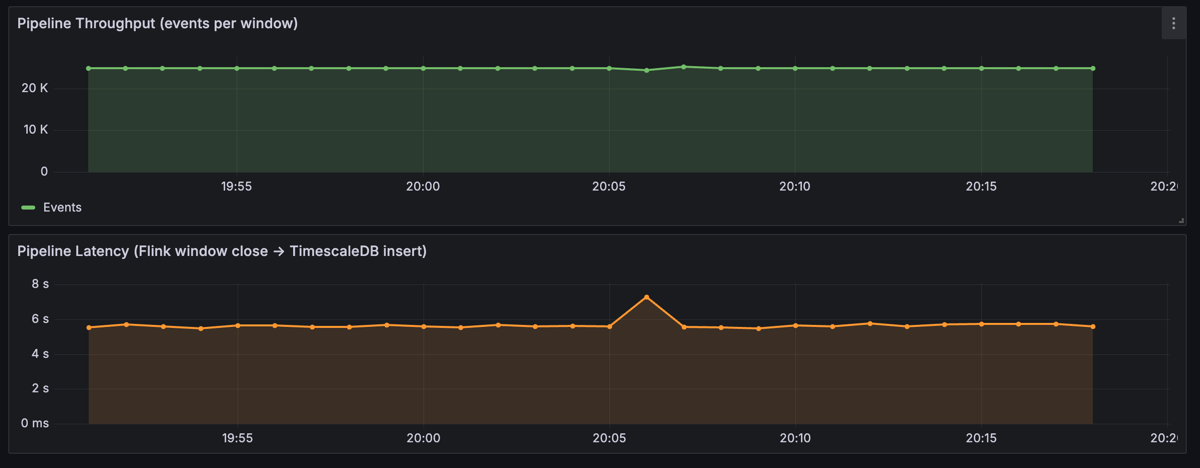
\includegraphics[width=\textwidth]{Figures/latency_throughput.png}
% %     \caption{Pipeline throughput and end-to-end latency under peak load.}
% %     \label{fig:latency-throughput}
% % \end{figure}
%
% \section{Alert Detection}
%
% % TODO: describe the test scenario — what readings you injected to trigger alerts
% Alert correctness was verified by replaying a sequence of readings with elevated pollutant concentrations designed to exceed the Z-score threshold. The Flink anomaly detection operator correctly identified onset conditions after ten consecutive anomalous windows and dispatched an alert email. Upon return to baseline readings, a recovery notification was issued after the corresponding ten-window recovery period. Figure~\ref{fig:alert-onset} and Figure~\ref{fig:alert-recovery} show the resulting alert emails captured in MailHog.
%
% \begin{figure}[H]
%     \centering
%     \begin{minipage}{0.48\textwidth}
%         \centering
%         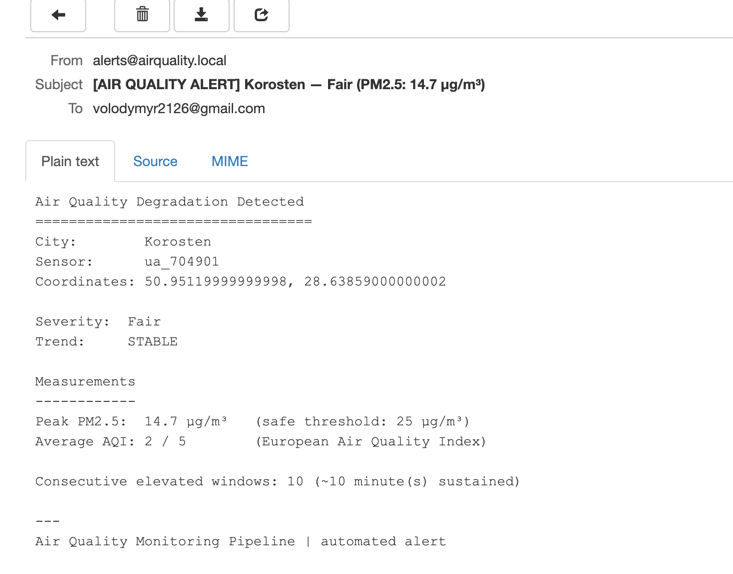
\includegraphics[width=\textwidth]{Figures/fair_alert_example.png}
%         \caption{Onset alert email triggered after sustained anomaly detection.}
%         \label{fig:alert-onset}
%     \end{minipage}
%     \hfill
%     \begin{minipage}{0.48\textwidth}
%         \centering
%         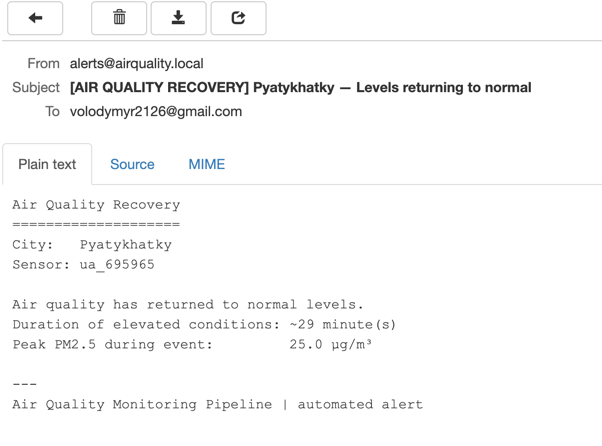
\includegraphics[width=\textwidth]{Figures/recovery_alert_example.png}
%         \caption{Recovery alert email triggered after return to baseline readings.}
%         \label{fig:alert-recovery}
%     \end{minipage}
% \end{figure}
%
% \section{Discussion}
%
% The results demonstrate that the implemented pipeline meets both primary objectives under the experimental conditions described. Several limitations of the evaluation should be noted. First, the data source is a replay of historical sensor readings rather than live hardware sensors, meaning network jitter and sensor failure scenarios are not represented. Second, all services were co-located on a single host, which eliminates network latency between components present in a distributed cloud deployment. At production scale — with ingestion distributed across Amazon MSK, processing on Amazon Managed Service for Apache Flink, and storage on Amazon RDS — latency characteristics would differ, though the architectural design preserves the same processing guarantees. Fault tolerance under node failure and cold-start recovery time were not measured and remain directions for future evaluation.
